\appendix

\section{Proofs}
\label{app:proofs}

For completeness we first recall two standard facts about DDPMs (which are not
contributions of this work). We then \emph{state and prove} the two standard
results relegated here from the main text to keep it focused---that the
subject-aware class contains the plain DDPM (Prop.~\ref{prop:contain}) and that
the noise-prediction error controls the reverse-step error
(Prop.~\ref{prop:prop})---together with the $x_0/\epsilon$ parameterization lemma
(Lemma~\ref{lem:x0eps}). Finally we prove the propositions of
Sections~\ref{sec:method_theory} and~\ref{sec:method_unify}.

\begin{lemma}[Closed-form forward marginal~\cite{ho2020ddpm}]
\label{lem:marginal}
With $\alpha_t=1-\beta_t$ and $\bar{\alpha}_t=\prod_{s=1}^{t}\alpha_s$, the forward
process of Eqs.~\eqref{eq:forward_chain}--\eqref{eq:forward_step} satisfies
$q(\mathbf{x}_t\mid\mathbf{x}_0)=\mathcal{N}\!\big(\mathbf{x}_t;\sqrt{\bar{\alpha}_t}\,\mathbf{x}_0,(1-\bar{\alpha}_t)\mathbf{I}\big)$.
\end{lemma}

\begin{proof}
Write the single-step update as
$\mathbf{x}_t=\sqrt{\alpha_t}\,\mathbf{x}_{t-1}+\sqrt{1-\alpha_t}\,\boldsymbol{\epsilon}_{t-1}$
with $\boldsymbol{\epsilon}_{t-1}\sim\mathcal{N}(\mathbf{0},\mathbf{I})$ i.i.d.
Unrolling one step gives
\[
\mathbf{x}_t=\sqrt{\alpha_t\alpha_{t-1}}\,\mathbf{x}_{t-2}
+\sqrt{\alpha_t(1-\alpha_{t-1})}\,\boldsymbol{\epsilon}_{t-2}
+\sqrt{1-\alpha_t}\,\boldsymbol{\epsilon}_{t-1}.
\]
The last two terms are independent zero-mean Gaussians with variances
$\alpha_t(1-\alpha_{t-1})$ and $1-\alpha_t$, which sum to
$1-\alpha_t\alpha_{t-1}$; hence they merge into a single
$\mathcal{N}\!\big(\mathbf{0},(1-\alpha_t\alpha_{t-1})\mathbf{I}\big)$ term.
Iterating down to $\mathbf{x}_0$ yields mean
$\big(\prod_{s=1}^{t}\sqrt{\alpha_s}\big)\mathbf{x}_0=\sqrt{\bar{\alpha}_t}\,\mathbf{x}_0$
and covariance $\big(1-\prod_{s=1}^{t}\alpha_s\big)\mathbf{I}=(1-\bar{\alpha}_t)\mathbf{I}$.
\end{proof}

\paragraph{Simplified training objective.}
Minimizing the variational bound on $-\log p_\theta(\mathbf{x}_0)$ reduces, after
the loss reweighting of Ho et al.~\cite{ho2020ddpm}, to the noise-prediction
objective $\mathcal{L}_{\text{simple}}$ of Eq.~\eqref{eq:lsimple}, which we use
throughout; see~\cite{ho2020ddpm} for the full derivation.

\begin{proof}[Proof of Proposition~\ref{prop:cond}]
Fix $t$ and abbreviate $g^\star=\mathbb{E}[\boldsymbol{\epsilon}\mid\mathbf{x}_t,t]$
and $h^\star=\mathbb{E}[\boldsymbol{\epsilon}\mid\mathbf{x}_t,t,S]$. By the tower
property of conditional expectation,
$g^\star=\mathbb{E}\!\big[h^\star\mid\mathbf{x}_t,t\big]$. Decompose the
subject-agnostic risk as
\[
R_u=\mathbb{E}\big\|\boldsymbol{\epsilon}-g^\star\big\|^2
=\mathbb{E}\big\|\boldsymbol{\epsilon}-h^\star\big\|^2
+\mathbb{E}\big\|h^\star-g^\star\big\|^2
+2\,\mathbb{E}\big\langle\boldsymbol{\epsilon}-h^\star,\,h^\star-g^\star\big\rangle .
\]
Conditioning the cross term on $(\mathbf{x}_t,t,S)$ and using
$\mathbb{E}[\boldsymbol{\epsilon}-h^\star\mid\mathbf{x}_t,t,S]=\mathbf{0}$, while
$h^\star-g^\star$ is $(\mathbf{x}_t,t,S)$-measurable, shows that the cross term
vanishes. Hence $R_u=R_c+\mathbb{E}\|h^\star-g^\star\|^2$. Finally, since
$g^\star=\mathbb{E}[h^\star\mid\mathbf{x}_t,t]$,
\[
\mathbb{E}\big\|h^\star-g^\star\big\|^2
=\mathbb{E}_{\mathbf{x}_t,t}\!\big[\operatorname{Var}_S\!\big(h^\star\mid\mathbf{x}_t,t\big)\big]\ge 0,
\]
which is~\eqref{eq:propcond}.
\end{proof}

\begin{proposition}[The subject-aware class contains the subject-agnostic DDPM]
\label{prop:contain}
Let $\mathcal{H}_u=\{\boldsymbol{\epsilon}^{c}_{\theta}(\mathbf{x}_t,t)\}$ be the
subject-agnostic denoiser class and let
$\mathcal{H}_c=\{\boldsymbol{\epsilon}^{c}_{\theta}(\mathbf{x}_t,t)+
\boldsymbol{\epsilon}^{s}_{\phi}(\mathbf{x}_t,t,\mathbf{e}(s))\}$ be the
dual-decoder FiLM-conditioned subject-aware class of Eq.~\eqref{eq:combined_epsilon}.
If the FiLM module can realize the identity modulation
$\boldsymbol{\gamma}(\mathbf{e})\equiv\mathbf{1}$,
$\boldsymbol{\delta}(\mathbf{e})\equiv\mathbf{0}$ and the individual branch can
output $\boldsymbol{\epsilon}^{s}_{\phi}\equiv\mathbf{0}$, then
$\mathcal{H}_u\subseteq\mathcal{H}_c$, and hence for any dataset
\begin{equation}
  \min_{h\in\mathcal{H}_c}\widehat{R}(h)\;\le\;\min_{h\in\mathcal{H}_u}\widehat{R}(h),
  \label{eq:contain}
\end{equation}
where $\widehat{R}$ is the empirical (training) risk. Subject-aware conditioning is
thus at least as expressive as a plain DDPM and can only lower the attainable
\emph{training} error; this concerns representational capacity, not the
generalization gap, which is why we regularize the embeddings
(Section~\ref{sec:exp_setup}).
\end{proposition}

\begin{proof}[Proof of Proposition~\ref{prop:contain}]
Setting $\boldsymbol{\gamma}(\mathbf{e})\equiv\mathbf{1}$ and
$\boldsymbol{\delta}(\mathbf{e})\equiv\mathbf{0}$ makes every FiLM layer
(Eq.~\eqref{eq:film}) the identity map $\mathbf{h}'=\mathbf{h}$, so the
conditioning input $\mathbf{e}(s)$ has no effect and
$\boldsymbol{\epsilon}_\theta(\mathbf{x}_t,t,\mathbf{e}(s))=\boldsymbol{\epsilon}_\theta(\mathbf{x}_t,t)$;
additionally taking $\boldsymbol{\epsilon}_\phi\equiv\mathbf{0}$ makes the
dual-decoder output coincide with the subject-agnostic denoiser. Hence every
element of $\mathcal{H}_u$ is realized by some element of $\mathcal{H}_c$, i.e.
$\mathcal{H}_u\subseteq\mathcal{H}_c$. The minimum of $\widehat{R}$ over a
superset is no larger than over the subset, which gives~\eqref{eq:contain}. (This
is a statement about representational capacity and empirical risk; it does not
bound the generalization gap.)
\end{proof}

\begin{proposition}[Noise-prediction error controls the reverse-step error]
\label{prop:prop}
Let $\widehat{\boldsymbol{\epsilon}}$ be the model's combined noise prediction
($\widehat{\boldsymbol{\epsilon}}=\widehat{\boldsymbol{\epsilon}}_{\theta,\phi}$
in \saddpm{}) and $\boldsymbol{\epsilon}^\star$ the true noise, with
$\|\widehat{\boldsymbol{\epsilon}}(\mathbf{x}_t,t)-\boldsymbol{\epsilon}^\star(\mathbf{x}_t,t)\|\le\eta_t$.
For the DDPM reverse mean
$\boldsymbol{\mu}_{\theta,\phi}(\mathbf{x}_t,t)=\tfrac{1}{\sqrt{\alpha_t}}\big(\mathbf{x}_t-\tfrac{\beta_t}{\sqrt{1-\bar{\alpha}_t}}\,\widehat{\boldsymbol{\epsilon}}(\mathbf{x}_t,t)\big)$
and the corresponding $\boldsymbol{\mu}^\star$ obtained by substituting the true
noise $\boldsymbol{\epsilon}^\star$, the reverse-step mean error satisfies, at the
same $\mathbf{x}_t$,
\begin{equation}
  \big\|\boldsymbol{\mu}_{\theta,\phi}(\mathbf{x}_t,t)-\boldsymbol{\mu}^\star(\mathbf{x}_t,t)\big\|
  =\frac{\beta_t}{\sqrt{\alpha_t}\,\sqrt{1-\bar{\alpha}_t}}\,\big\|\widehat{\boldsymbol{\epsilon}}-\boldsymbol{\epsilon}^\star\big\|
  \;\le\;\frac{\beta_t}{\sqrt{\alpha_t}\,\sqrt{1-\bar{\alpha}_t}}\;\eta_t.
  \label{eq:prop}
\end{equation}
Since $\boldsymbol{\mu}$ is affine in $\widehat{\boldsymbol{\epsilon}}$, the
relation is an exact identity (hence tight): the noise-prediction loss
$\mathcal{L}_r$ directly governs the per-step reconstruction error, with step gain
$c_t=\beta_t/(\sqrt{\alpha_t}\sqrt{1-\bar{\alpha}_t})$. Summing per-step deviations
along a reference trajectory bounds the cumulative mean error by
$\sum_t c_t\eta_t$; a fully end-to-end bound would additionally require a
Lipschitz/contraction assumption on the reverse kernel, which we do not claim.
\end{proposition}

\begin{proof}[Proof of Proposition~\ref{prop:prop}]
Both $\boldsymbol{\mu}_\theta$ and $\boldsymbol{\mu}^\star$ use the same
$\mathbf{x}_t$ and differ only through the noise term, which enters affinely.
Subtracting,
\[
\boldsymbol{\mu}_\theta(\mathbf{x}_t,t)-\boldsymbol{\mu}^\star(\mathbf{x}_t,t)
=-\frac{1}{\sqrt{\alpha_t}}\cdot\frac{\beta_t}{\sqrt{1-\bar{\alpha}_t}}\,
\big(\widehat{\boldsymbol{\epsilon}}(\mathbf{x}_t,t)-\boldsymbol{\epsilon}^\star(\mathbf{x}_t,t)\big),
\]
since the $\mathbf{x}_t$ terms cancel. Taking norms gives the equality
in~\eqref{eq:prop}, and applying
$\|\widehat{\boldsymbol{\epsilon}}-\boldsymbol{\epsilon}^\star\|\le\eta_t$ gives
the bound. The coefficient $c_t=\beta_t/(\sqrt{\alpha_t}\sqrt{1-\bar{\alpha}_t})$
is a fixed positive scalar, so the relation is tight.
\end{proof}

\begin{proof}[Proof of Proposition~\ref{prop:orth}]
Because the columns of $\mathbf{Z}^{c}$ and $\mathbf{Z}^{s}$ are mean-centered,
the empirical cross-covariance of the two feature sets is
$\widehat{\mathrm{Cov}}(\mathbf{z}^{c},\mathbf{z}^{s})=\tfrac{1}{B}{\mathbf{Z}^{c}}^{\!\top}\mathbf{Z}^{s}$.
Therefore
\[
\mathcal{L}_o=\big\|{\mathbf{Z}^{c}}^{\!\top}\mathbf{Z}^{s}\big\|_F^2
=B^2\big\|\widehat{\mathrm{Cov}}(\mathbf{z}^{c},\mathbf{z}^{s})\big\|_F^2\ge 0,
\]
which equals zero if and only if every entry of the cross-covariance matrix is
zero, i.e., the content and subject features are pairwise uncorrelated.
Minimizing $\mathcal{L}_o$ thus enforces second-order decorrelation; note that
decorrelation does not in general imply statistical independence.
\end{proof}

\begin{proof}[Proof of Proposition~\ref{prop:da}]
This is the bound of Ben-David et al.~\cite{bendavid2010theory} (their
Theorem~2), applied with the source and target distributions taken to be the
content-representation distributions $P^{c}_S,P^{c}_T$ induced by $D_\theta$; we
restate it here only for reference and claim no novelty. The multi-class
extension follows analogously with a discrepancy-style divergence in place of
$d_{\mathcal{H}\Delta\mathcal{H}}$.
\end{proof}

\begin{proof}[Proof of Proposition~\ref{prop:obs}]
The argument mirrors that of Proposition~\ref{prop:cond} with $\mathbf{y}$ in
place of $(\mathbf{x}_t,t)$. Abbreviate
$\bar{g}=\mathbb{E}[\mathbf{x}_0\mid\mathbf{y}]$ and
$\bar{h}=\mathbb{E}[\mathbf{x}_0\mid\mathbf{y},S]$; by the tower property
$\bar{g}=\mathbb{E}[\bar{h}\mid\mathbf{y}]$. Expanding
$\bar{R}_u=\mathbb{E}\|\mathbf{x}_0-\bar{g}\|^2$ and noting that the cross term
$\mathbb{E}\langle\mathbf{x}_0-\bar{h},\,\bar{h}-\bar{g}\rangle$ vanishes
(condition on $(\mathbf{y},S)$: $\mathbb{E}[\mathbf{x}_0-\bar{h}\mid\mathbf{y},S]=\mathbf{0}$
while $\bar{h}-\bar{g}$ is $(\mathbf{y},S)$-measurable) gives
$\bar{R}_u=\bar{R}_c+\mathbb{E}\|\bar{h}-\bar{g}\|^2$, and
$\mathbb{E}\|\bar{h}-\bar{g}\|^2=\mathbb{E}_{\mathbf{y}}[\operatorname{Var}_S(\bar{h}\mid\mathbf{y})]$,
which is~\eqref{eq:obs}. The gap is zero iff $\bar{h}$ is $\mathbf{y}$-measurable,
i.e.\ $\bar{h}(\mathbf{y},S)=\bar{g}(\mathbf{y})$ a.s.; if $\mathbf{x}_0=f(\mathbf{y})$
for some measurable $f$ (shared artifact) then $\bar{h}=\bar{g}=f$ and the gap
vanishes, whereas a subject-specific artifact makes $\bar{h}$ depend on $S$ and the
gap positive.
\end{proof}

\begin{proof}[Proof of Proposition~\ref{prop:joint}]
Since $\mathbf{y}_c$ is a sub-vector of $\mathbf{y}_{1:C}$, the conditional
expectation given the larger collection is the $L^2$ projection onto a larger
subspace, so for each $c$,
$\mathbb{E}\|\mathbf{x}_{0,c}-\mathbb{E}[\mathbf{x}_{0,c}\mid\mathbf{y}_{1:C}]\|^2\le
\mathbb{E}\|\mathbf{x}_{0,c}-\mathbb{E}[\mathbf{x}_{0,c}\mid\mathbf{y}_c]\|^2$, with
gap $\mathbb{E}_{\mathbf{y}_c}[\operatorname{Var}(\mathbb{E}[\mathbf{x}_{0,c}\mid\mathbf{y}_{1:C}]\mid\mathbf{y}_c)]$
by the same tower-property decomposition as Proposition~\ref{prop:cond}. Summing
over $c$ gives~\eqref{eq:joint}; the gap is strictly positive whenever the other
channels are informative about $\mathbf{x}_{0,c}$ given $\mathbf{y}_c$, i.e.\ when
the artifact has cross-channel structure.
\end{proof}

\begin{lemma}[$x_0$- and $\epsilon$-parameterization]
\label{lem:x0eps}
The $x_0$- and $\epsilon$-parameterizations of the reverse mean are related by the
affine bijection
$\mathbf{x}_0=(\mathbf{x}_t-\sqrt{1-\bar{\alpha}_t}\,\boldsymbol{\epsilon})/\sqrt{\bar{\alpha}_t}$;
hence they share the same Bayes-optimal predictor and differ only in the per-step
weighting of the training loss.
\end{lemma}

\begin{proof}[Proof of Lemma~\ref{lem:x0eps}]
For fixed $(\mathbf{x}_t,t)$ the map
$\boldsymbol{\epsilon}\mapsto\mathbf{x}_0=(\mathbf{x}_t-\sqrt{1-\bar{\alpha}_t}\,\boldsymbol{\epsilon})/\sqrt{\bar{\alpha}_t}$
is an affine bijection, so a predictor of one quantity induces a predictor of the
other with the same conditional expectation; the Bayes-optimal solutions coincide.
Substituting the relation into the squared-error objective rescales the per-step
loss by $(1-\bar{\alpha}_t)/\bar{\alpha}_t$, so the two parameterizations optimize
the same risk under different per-timestep weights.
\end{proof}

\section{Additional Results: EMG Artifacts and Spectral Recovery}
\label{app:figures}

Figures~\ref{fig:f2emg}--\ref{fig:f6emg} provide the myogenic (EMG) counterparts
of the main-text ocular (EOG) results, together with the spectral-recovery view.
EMG is a broadband artifact and is harder than EOG, as the single-channel
benchmark (Figure~\ref{fig:f2emg}) shows.

\begin{figure}[t]
  \centering
  
\includegraphics[width=\linewidth]{figures/F2_metrics_vs_snr_EMG}
  \caption{Single-channel denoising on the EEGdenoiseNet benchmark (EMG; cf.\
  Figure~\ref{fig:f2}). For the harder broadband myogenic artifact, \saddpmcond{}
  trails the supervised CNNs (mean CC $0.680$ vs.\ SimpleCNN $0.742$).}
  \label{fig:f2emg}
  \Description{Three line plots versus input SNR for the EMG artifact; the
  SADDPM-Cond correlation-coefficient curve sits somewhat below the SimpleCNN and
  NovelCNN curves.}
\end{figure}

\begin{figure}[t]
  \centering
  
\includegraphics[width=\linewidth]{figures/F1_waveforms_EMG}
  \caption{Example EMG-contaminated segments at four input SNRs (cf.\
  Figure~\ref{fig:f1}).}
  \label{fig:f1emg}
  \Description{Four stacked time-series panels; the denoised trace follows the
  clean trace while the broadband myogenic noise in the contaminated trace is
  reduced.}
\end{figure}

\begin{figure}[t]
  \centering
  
\includegraphics[width=\linewidth]{figures/F5_multichannel_EMG}
  \caption{Multi-channel joint denoising for the laterally distributed myogenic
  artifact (cf.\ Figure~\ref{fig:f5}); joint denoising reaches CC $\approx0.99$.}
  \label{fig:f5emg}
  \Description{A scalp topomap with a laterally distributed myogenic artifact and
  three channel-by-time heatmaps showing contaminated, denoised, and clean
  22-channel windows.}
\end{figure}

\begin{figure}[t]
  \centering
  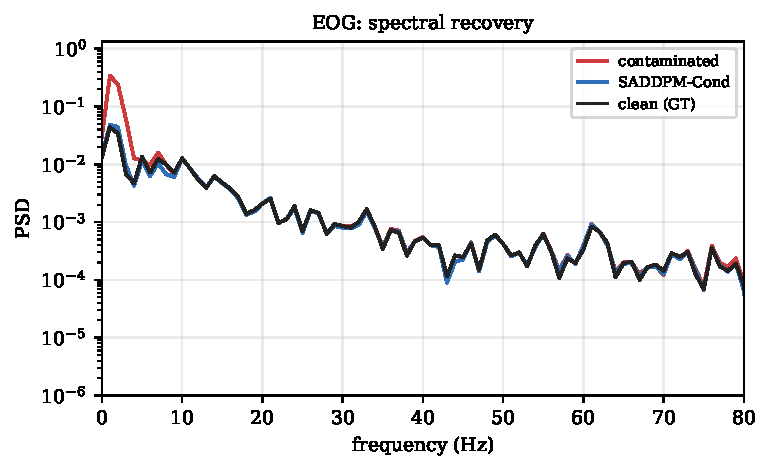
\includegraphics[width=\linewidth]{figures/F6_psd_EOG}
  \caption{Spectral recovery (EOG): the \saddpmcond{}-denoised power spectral
  density (blue) matches the clean spectrum (black), removing the excess
  low-frequency power introduced by the ocular artifact (red).}
  \label{fig:f6eog}
  \Description{A power spectral density plot; the contaminated spectrum has excess
  power below 5 Hz, while the denoised spectrum matches the clean spectrum across
  frequencies.}
\end{figure}

\begin{figure}[t]
  \centering
  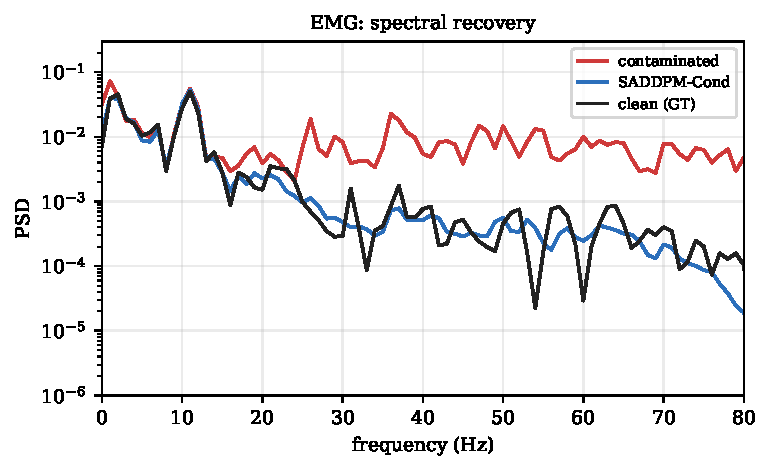
\includegraphics[width=\linewidth]{figures/F6_psd_EMG}
  \caption{Spectral recovery (EMG; cf.\ Figure~\ref{fig:f6eog}).}
  \label{fig:f6emg}
  \Description{A power spectral density plot for the EMG case; the denoised
  spectrum matches the clean spectrum.}
\end{figure}
